\documentclass{article}
\usepackage[final]{neurips_2021}

\usepackage[utf8]{inputenc} % allow utf-8 input
\usepackage[T1]{fontenc}    % use 8-bit T1 fonts
\usepackage{hyperref}       % hyperlinks
\usepackage{url}            % simple URL typesetting
\usepackage{booktabs}       % professional-quality tables
\usepackage{amsfonts}       % blackboard math symbols
\usepackage{nicefrac}       % compact symbols for 1/2, etc.
\usepackage{microtype}      % microtypography
\usepackage{xcolor}         % colors
\usepackage{lipsum}
\usepackage{amsmath}
\usepackage{setspace}
\usepackage{bbm}
\usepackage[linesnumbered,ruled,commentsnumbered]{algorithm2e}
\usepackage{parskip}
\usepackage{graphicx}
\usepackage{caption}
\usepackage{subcaption}

\graphicspath{{./figures/active/neural/}}
\IncMargin{1.5em}

\title{Active Heirarchical Metric Learning}

\author{
  Nicolas Beltran\\
  Department of Computer Science\\
  Columbia University\\
  New York City, NY 10027 \\
  \texttt{nb2838@columbia.edu}\\
  \And
  Ketan Jog\\
  Department of Computer Science\\
  Columbia University\\
  New York City, NY 10027 \\
  \texttt{kj2473@columbia.edu}\\
}


\begin{document}

\maketitle

\begin{abstract}
    Many problems require a well defined notion of a distance between points in space.
    Constructing or finding such a measure falls into the field of metric learning.
    Although many algorithms exist in the field when a learner has access to a fixed dataset,  there is room for improvement in terms of samples efficiency that the learner needs to know, imposition of desired structure, especially when the data appears in an \textit{online} manner.
    We propose a project that reduces the problem of online/active metric learning to bandits. In case our plan turn out to be too ambitious, we have a fallback - an empirical investigation of some algorithms that have dealt with the problem in an online setting or in situations where the learner can selective query the points that it wants to know information about.
\end{abstract}


\section{Introduction}

\section{Related Work}

\section{Long-term goals}

\section{Preliminaries}


% --------------------------------------------------------------
% --------------------------------------------------------------
\section{Problem Statement}
\label{problem-statement}
% --------------------------------------------------------------
% --------------------------------------------------------------
We consider two different problems.
The first problem consists of making a series of sequential predictions while learning a
similiarity measure. We refer to this problem as online similarity prediction.
The second problem consists of learning a similarity measure while querying points in space.
We refer to this problem as active similarity learning.
A precise description of both problems is provided below.

\subsection{Online similarity learning}
\label{problem-statement:online-similarity-learning}
We consider an online similarity learning problem played over $T$ rounds.
At round $t$ the environment samples $K$ pairs of points $(\mathbf{x}_{t,k}^1, \mathbf{x}_{t,k}^2) \in \mathbb{R}^{2n}$.
The agent then chooses pair $k_t \in [K]$ and is given a reward $r_{t,k_{t}} \in \{1, -1\}$.
We assume that there exists some similarity function unknown to the agent $\phi: \mathbb{R}^{2n} \to \{-1, 1 \}$
and that the rewards are such that if at time $t \in [T]$ the agent chooses pair $(\mathbf{x}_{t,k}^1, \mathbf{x}_{t,k}^2)$
then the reward is $\phi(\mathbf{x}_{t,k}^1, \mathbf{x}_{t,k}^2)$.

As usual we define the regret as
\[ R_T = \mathbb{E}\left[\sum_{t =1}^T \phi(\mathbf{x}_{t,k^\star_t}^1, \mathbf{x}_{t,k^\star_t}^2) - \phi(\mathbf{x}_{t,k_t}^1, \mathbf{x}_{t,k_t}^2)\right]\]
where $k_t^\star = \text{argmax}_{k\in [K]} \phi(\mathbf{x}_{t,k}^1, \mathbf{x}_{t,k}^2)$

\subsection{Active similarity learning}
\label{problem-statement:active-similarity-learning}
We assume that the learner has access to a dataset $D = \{\mathbf{x}_i \in \mathbb{R}^n| i \in [N]\}$ of unlabeled points and that there exists some function $\phi: \mathbb{R}^{2n} \to \{-1, 1\}$ which the learner is trying to learn.
The learner can query $T$ pairs of points in this set $D$ to obtain a dataset $D_T = \{(\mathbf{x}_t^1, \mathbf{x}_t^2, y_t) ~|  ~t \in [T]\}$ . We assume that the learner mantains and estimate $\hat{\phi}_t \in \mathcal{F}$ of $\phi$, where $\mathcal{F}$ is its function class  and denote the loss between an estimate $\hat{\phi}$ a $\phi$ as
\[ \mathcal{L}(\phi, \hat{\phi}) = \mathbb{E}_\mathcal{(\mathbf{x}, \mathbf{y}) \sim \mathcal{D} \times \mathcal{D}}[(\hat{\phi}(\mathbf{x},\mathbf{y}) - \phi(\mathbf{x}, \mathbf{y}))^2] \]
It's objective is to find $\min_{\phi \in \mathcal{F}} \mathcal{L}(\hat{\phi}_T, \phi)$


\section{Description of the algorithms}
In total we provide 4 different algorithms which we describe below.
However, in reality they can be thought of as 2 different algorithms (a neural and linear model for similarity)  which contain slight modifications to accomodate for the online similarity learning problem and the active similarity learning problem.
We refer to our algorithms as OnSim-LinUCB, ActSim-LinUCB,OnSim-NeuralUCB, ActSim-NeuralUCB, depeding on whether they are based on LinUCB or NeuralUCB and on whether they attempt to solve the active or online formulation of our problem.
We provide the four versions below with their slightly different modifications for completeness.


\subsection{Online similarity learning}
For our problem of online similarity learning we adopt the frameworks of  LinUCB  as described in \cite{linucb} and  NeuralUCB as described in \cite{neuralucb}. We explain this in detail below.

\subsubsection{OnSim-LinUCB}
Our first algorithm performs a straighforward reduction of the online similarity learning problem to that of regular contextual bandits. We do this by assuming a linear structure on the similarity.

Mathematically, if we adopt the formulation we proposed above (\ref{problem-statement:online-similarity-learning}), we choose to model the similarity of two points as  $\phi(\mathbf{x}, \mathbf{y}) = \mathbf{x}^\top \mathbf{A} \mathbf{y}$.
We can see that this is a reasonable thing to do if we consider that
\[\phi(\mathbf{x}, \mathbf{y}) = \mathbf{x}^\top \mathbf{A} \mathbf{y} = \sum_{i =1}^n\sum_{j=1}^n \mathbf{x}_i \mathbf{y}_j \mathbf{A}_{i,j} \]
which we is linear in $\mathbf{A}$ and thus allows us to use the framework of LinUCB for our problem.
Attending to this fact, one can see that Algorithm \ref{algo:onsim-linucb} is almost identical to the first algorithms in \cite{linucb}.
\begin{algorithm}
  \label{algo:onsim-linucb}
  \setstretch{1.2}
    \SetKwInOut{Input}{Input}
    \Input{Rounds $T$ and exploration parameter $\alpha$}
    $A \gets I_{n^2}$\;
    $b \gets 0_{n^2}$\;
    \For{$t \in [T]$}{
      $\theta_t \gets A^{-1}b$
      Observe $K$ pairs of vectors $x^k \in \mathbb{R}^n$, $y^k \in \mathbb{R}^n$\;
      Create $z_{t,k} = (x_1^ky_1^k, x_1^ky_1^k, \dots, x_n^k y_{n-1}^k, x_n^k y_n^k)$\;
      \For{$k \in [K]$}{
        $p_{t,a} \gets \theta_t^\top z_{t,k} + \alpha \sqrt{z_{t,k} A^{-1} x_{t,a}}$
      }
      Choose action $a_t = \text{argmax}_ap_{t,a}$ with ties broken arbitrarily\;
      Observe payoff $ r_t \in \{-1,1 \}$\;
      $A \gets A + z_{t,a_t}z_{t,a_t}^\top$\;
      $b \gets z_{t,a_t}r_t$\;
    }
    \caption{OnSim-LinUCB}
\end{algorithm}

\subsubsection{OnSim-NeuralUCB}
Unsurprisingly, the expressive power of the above framework is quite limited.
The limitation comes from the fact that Algorithm \ref{algo:onsim-linucb} essentially assumes that similarity is the result
of a dot prouct in which both points are independently mapped to a new representation via a linear transformation. This will obviously not be true for many datasets.
To overcome these limitations we adapt NeuralUCB \cite{neuralucb} to our circumstances.

Formally, we assume that\footnote{It is also possible to assume that we don't normalize the last inner product, we refer to this verision and unormalized NeuralUCB. We provide some comparisons of this verison also below.}
\[ \phi(x,y) = \cos\left(f(x;\mathbf{\theta}), f(y;\mathbf{\theta})\right) = \frac{\langle f(x;\mathbf{\theta}), f(y;\mathbf{\theta}) \rangle}{||f(x;\mathbf{\theta})||_2 ||f(y;\mathbf{\theta})||_2}\]
Here $f: \mathbb{R}^n \to \mathbb{R}^m$ is a simple neural network of the form
\[ f(x; \theta) = b_L + W_{L} \sigma\left(b_{L-1} +  W_{L-1} \sigma\left( \dots \sigma\left(b_1 + W_1 x\right)\right) \right)\]
for some $L \in \mathbb{N}_{\geq 2}$, $W_1 \in \mathbb{R}^{d \times n}$, $W_{L} \in \mathbb{R}^{m \times d}$, $W_{l} \in \mathbb{R}^{d\times d}$ if $l \in [2, L-1]$, $b_L \in \mathbb{R}^m$, $b_l \in \mathbb{R}^d$ for $l \neq L$, and where $\sigma(x) = \max\{0, x\}$ applied component wise. We use $\theta$ to denote the flattened vector of $(W_L, b_L, \dots, W_1, b_1)$.
Using this notation OnSim-NeuralUCB is described below in Algorithm \ref{algo:onsim-neuralucb}. We use $p$ to denote the total number of trainable parameters in the neural network.

\begin{algorithm}
  \label{algo:onsim-neuralucb}
  \setstretch{1.2}
    \SetKwInOut{Input}{Input}
    \Input{Rounds $T$, exploration parameter $\alpha$, $\tau_r$ frequency of resets, $\tau_T$ frequency of training, $E$ epochs for training, $b_s$ batch size for training, $\epsilon$ learning rate.}
    $A \gets I_{p}$\;
    \For{$t \in [T]$}{
      Observe $K$ pairs of vectors $x_t^k \in \mathbb{R}^n$, $y_t^k \in \mathbb{R^n}$\;
      \For{$k \in [K]$}{
        $p_{t,k} \gets \phi(x,y) + \alpha \sqrt{(\nabla_\theta \phi(x_t^k, y_t^k))^\top A^{-1}\nabla_\theta\phi(x_t^k,y_t^k)}$\;
      }
      Choose pair $k_t = \text{argmax}_kp_{t,k}$ with ties broken arbitrarily\;
      Observe payoff $ r_t \in \{-1,1 \}$\;
      \If{$t \mod \tau_r = 0$ }{
        $\theta \gets \text{Train}(\epsilon,E, \{(x_i^{k_i}, y_i^{k_i}, r_i)\}_{i=1}^t,b_s)$\;
      }
      \If{$t \mod \tau_T = 0$ }{
        $A \gets I_p$
      }
      $A \gets A + \nabla_\theta \phi(x_t^k, y_t^k)(\nabla_\theta\phi(x_t^k,y_t^k))^\top$\;
    }
    \caption{OnSim-NeuralUCB}
  \end{algorithm}

Intuitively, this algorithm acts optimally with the current set of parameters that it is given and every so often it stops back to train the network. In Algorithm \ref{algo:train} we simply describe the normal process for training a classifier with mean squared error loss and assume that a normal gradient based algorithm is used.
In the description we use Stochastic Gradient Descent as done in \cite{neuralucb} but we believe that despite lack of theoretical justification, more modern optimization strategies such as Adam \cite{adam} do a better job in practice.

Although our algorithm is very similar to that proposed in \cite{neuralucb} it differs in some key aspects.
First, and perhaps most importantly, we adopt a very different architecture from that proposed in the original paper.
In it, the authors assume that the layers of the neural network have no bias, assume a particular initialization scheme, don't use a cosine similarity function at the end of the neural network, nor do they implement a siamese network as we do.
Second, we restart $A$ throughout training. Third, we use a constant exploration parameter throughout the duration of the algorithm.

We propose these changes because we believe they are more sensible for our particular application (and do provide better empirical performance) but they destroy the theoretical guarantees provided by original paper in which they were used, alongside arguments to the  neural tangent kernel matrix \cite{neuraltangentkernel} to provide a $\tilde{O}(\sqrt{T})$, bound on the regret of algorithm.

\begin{algorithm}
  \label{algo:train}
  \setstretch{1.2}
    \SetKwInOut{Input}{Input}
    \Input{$\epsilon$ learning rate, $E$ number of epochs, dataset $\{(x_i^{k_i}, y_i^{k_i}, r_i)\}_{i=1}^t$, $b_s$ batch size}

    optimizer $\gets$ SGD($\epsilon, \theta$)\;
    \For{$j = 1, \dots, E$}{
      $\mathcal{D} \gets \{(x_1^{k_1}, y_1^{k_1}, r_1), \dots, (x_t^{k_t}, y_t^{k_t}, r_t)$ \;
      \While{$\mathcal{D}$ is not empty}{
        Sample minibatch $M$ of size $b_s$ from the training examples\;
        $l = \frac{1}{M}\sum_{(x_i^{k_{i}}, y_i^{k_i}, r_i) \in M} (\phi(x_i^{k_{i}}, y_i^{k_i}) - r_i)^2$\;
        $\theta \gets$ update using optimizer with loss $l$\;

        Remove $M$ from $\mathcal{D}$\;
      }
    }
    \caption{Train}
  \end{algorithm}

  \subsection{Active Similarity Learning}
  Despite the differences with online similarity learning, for the active version of the problem we modify the above algorithms only slightly.
  The idea is to use the optimism bonus as a measure of uncertainty and ignore completely the reward.
  Using this framework, each time we have to make a query we can simply sample uniformly a subset of points in the unlabeled dataset $\mathcal{D}$  and then we reveal the label of the pair with the highest uncertainty as measured by the bonus.
  Although we use the bandits notation that we were using above, it is important to emphasize that $r$ no longer represents a reward but rather the labels for the similarity of the points themselves.
  Algorithms \ref{algo:active-neuralucb} and \ref{algo:active-linucb} describe these processes formally.
  In Algorithm \ref{algo:active-neuralucb} the most important change is line \ref{change:active-neuralucb} and in algorithm
  \ref{algo:active-linucb} the most important change is line \ref{change:active-linucb}.
  \begin{algorithm}
  \label{algo:active-neuralucb}
  \setstretch{1.2}
    \SetKwInOut{Input}{Input}
    \Input{Queries $T$, exploration parameter $\alpha$, $\tau_r$ frequency of resets, $\tau_T$ frequency of training, $E$ epochs for training, $b_s$ batch size for training, $\epsilon$ learning rate.}
    $A \gets I_{p}$\;
    \For{$t \in [T]$}{
      Sample $K$ pairs of vectors $x_t^k \in \mathbb{R}^n$, $y_t^k \in \mathbb{R}^n$ from dataset $D$\;
      \For{$k \in [K]$}{
        $p_{t,k} \gets \alpha \sqrt{(\nabla_\theta \phi(x_t^k, y_t^k))^\top A^{-1}\nabla_\theta\phi(x_t^k,y_t^k)}$\;
        \label{change:active-neuralucb}
      }
      Choose pair $k_t = \text{argmax}_kp_{t,k}$ with ties broken arbitrarily\;
      Query label $ r_t \in \{-1,1\}$\;
      \If{$t \mod \tau_r = 0$ }{
        $\theta \gets \text{Train}(\epsilon,E, \{(x_i^{k_i}, y_i^{k_i}, r_i)\}_{i=1}^t,b_s)$\;
      }
      \If{$t \mod \tau_T = 0$ }{
        $A \gets I_p$
      }
      $A \gets A + \nabla_\theta \phi(x_t^k, y_t^k)(\nabla_\theta\phi(x_t^k,y_t^k))^\top$\;
    }
    \caption{Active-NeuralUCB}
  \end{algorithm}


\begin{algorithm}
  \label{algo:active-linucb}
  \setstretch{1.2}
    \SetKwInOut{Input}{Input}
    \Input{Rounds $T$ and exploration parameter $\alpha$}
    $A \gets I_{n^2}$\;
    $b \gets 0_{n^2}$\;
    \For{$t \in [T]$}{
      $\theta_t \gets A^{-1}b$
      Observe $K$ pairs of vectors $x^k \in R^n$, $y^k \in R^n$\;
      Create $z_{t,k} = (x_1^ky_1^k, x_1^ky_1^k, \dots, x_n^k y_{n-1}^k, x_n^k y_n^k)$\;
      \For{$k \in [K]$}{
        $p_{t,a} \gets  \alpha \sqrt{z_{t,k} A^{-1} x_{t,a}}$
        \label{change:active-linucb}
      }
      Choose action pair $k_t = \text{argmax}_ap_{t,a}$ with ties broken arbitrarily.\;
      Observe label $ r_t \in \{-1,1 \}$\;
      $A \gets A + z_{t,a_t}z_{t,a_t}^\top$\;
      $b \gets z_{t,a_t}r_t$\;
    }
    \caption{Active-LinUCB}
\end{algorithm}
\section{Empirical Evaluation}
Below we describe the set of experiments that we performed.
We test separately NeuralUCB and LinUCB based algorithms as we logically expect them to perform
very differently due to the limitations of a linear approach.

\subsection{NeuralUCB}

\paragraph{Dataset}
Although we tested on various datasets including MNIST, CIFAR-10 and crescent moons
we found that the algorithm was impractical to use on the first two due to the expensive computation
of the matrix operation.
To reduce the dimension we had to apply PCA, however because this process implicitely leads to a better representation
useful for our scenarios, we opted not to include the results here an only focus on the performance of crescent moons.
However, these experiments can be found on the associated github repo.

\paragraph{Neural Network}
For our experiments we used a simple 3 layer neural network with 25 hidden units in each layer and an output dimension of 2.
In addition to the description of the algorithm provided above, we also added a dropout layer after each regular layer of the neural network with
$p =0.3$. We found this to be an important in practice so that the neural network would not overfit in the low data situation that it was operating in.

\paragraph{Optimizer}
We attempted to use SGD, Adam, and SGD with momentum with various different hyper parameters.
Generally, We found that Adam was the best performing optimizer followed by SGD with momentum.
When appropiate we report the results for SGD with momentum and Adam and when non is mentioned we report the results for Adam.
We found that the defaults for Adam in \cite{adam} worked well for our experiments.

We used Adam with learning rate $0.001$ and the default hyper-parameters suggested by the original paper \cite{adam}.
We also attempted to use other optimizations like SGD or SGD with momentum but overall found the performance of Adam to be
significantly better.
When appropiate we report additional results for comparison but we report the results for Adam when an optimizer is not mentioned.

\subsubsection{Experiment 1: Effectiveness of a linear classifier on learned features}
To determine the quality of our embeddings we used a linear classifier to classify the learned features and observe these values
per iteration. We report the results both for SGD with momentum and Adam. Additionally, we also report the performance of NeuralUCB
using the unormalized version of cosine similarity. All graphs contain the mean and a 95\% confidence interval
computed over 10 runs of the algorithm. The results are shown in Figures (\ref{fig:svm-non-normalized-ci}) and (\ref{fig:svm-normalized-ci})

% add figures
\begin{figure}[!h]
  \centering
  \begin{minipage}{.55\textwidth}
    \centering
    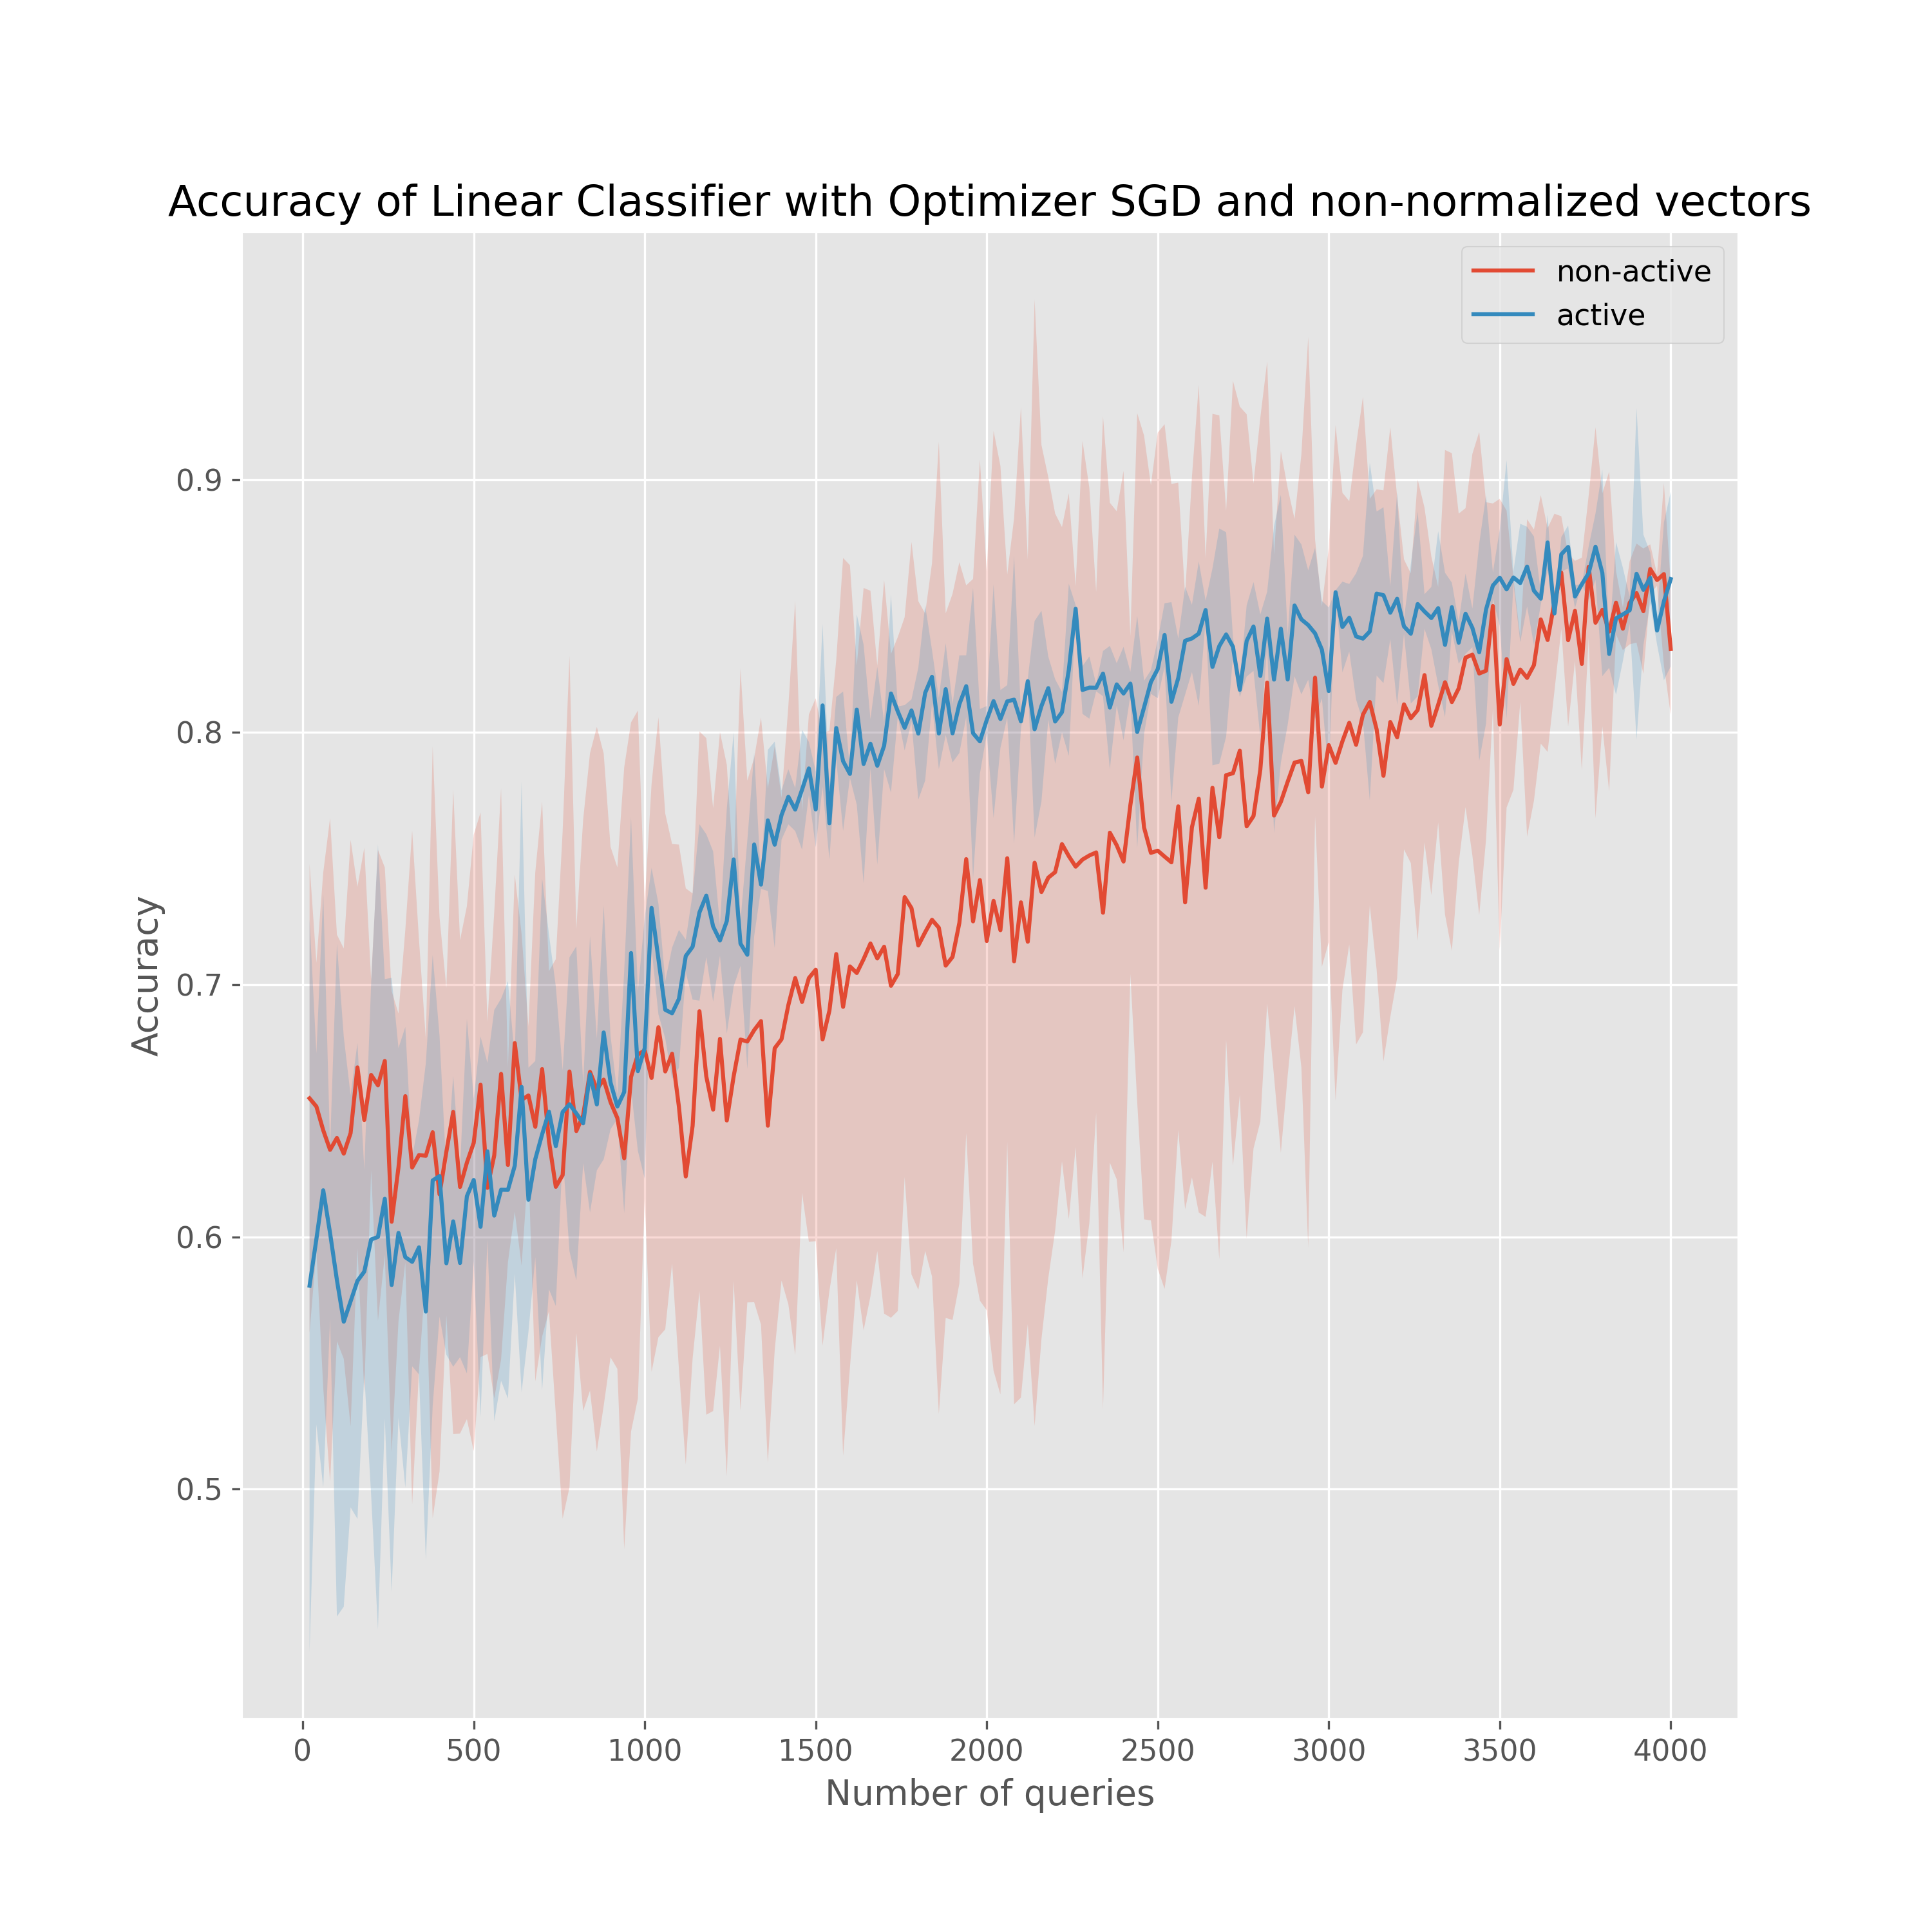
\includegraphics[width=\linewidth]{active-vs-base-moons-linear-loss-SGD-non-normalized-ci}
  \end{minipage}%
  \begin{minipage}{.55\textwidth}
    \centering
    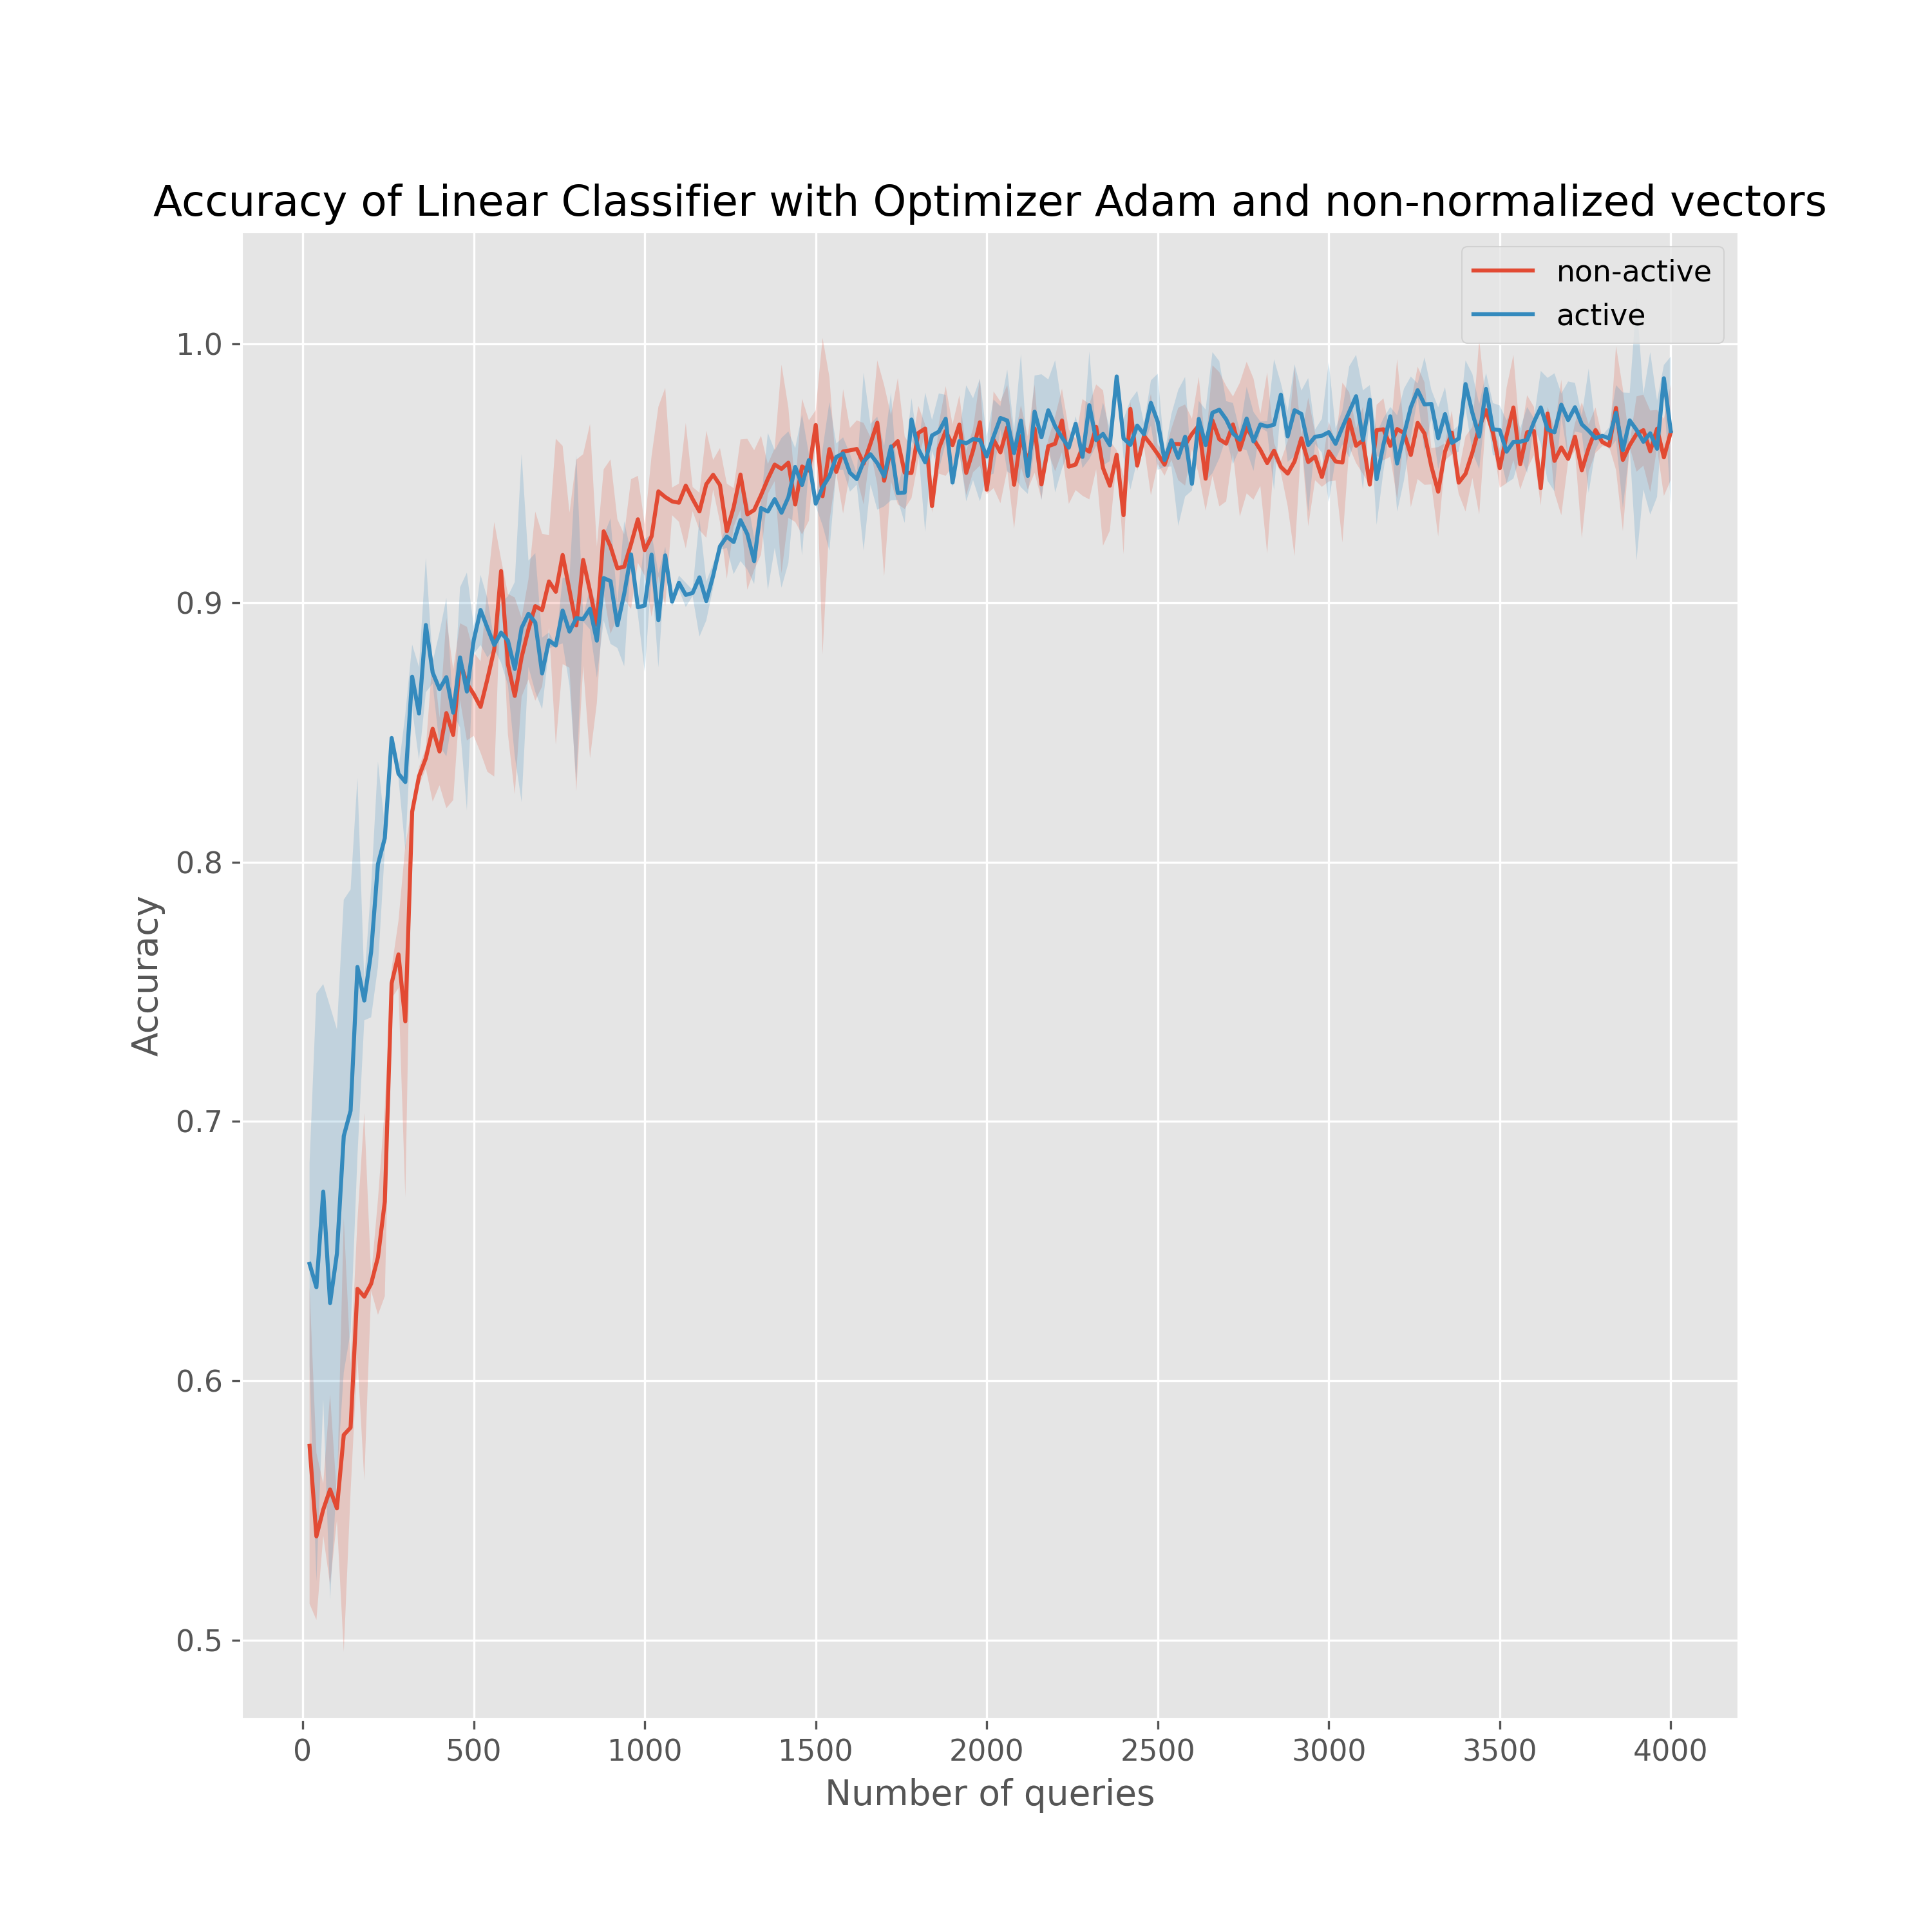
\includegraphics[width=\linewidth]{active-vs-base-moons-linear-loss-Adam-non-normalized-ci}
  \end{minipage}
  \caption{Performance SVM on non-normalzied learned features Adam vs SGD}
  \label{fig:svm-non-normalized-ci}
\end{figure}

% add figures
\begin{figure}[!h]
  \centering
  \begin{minipage}{.55\textwidth}
    \centering
    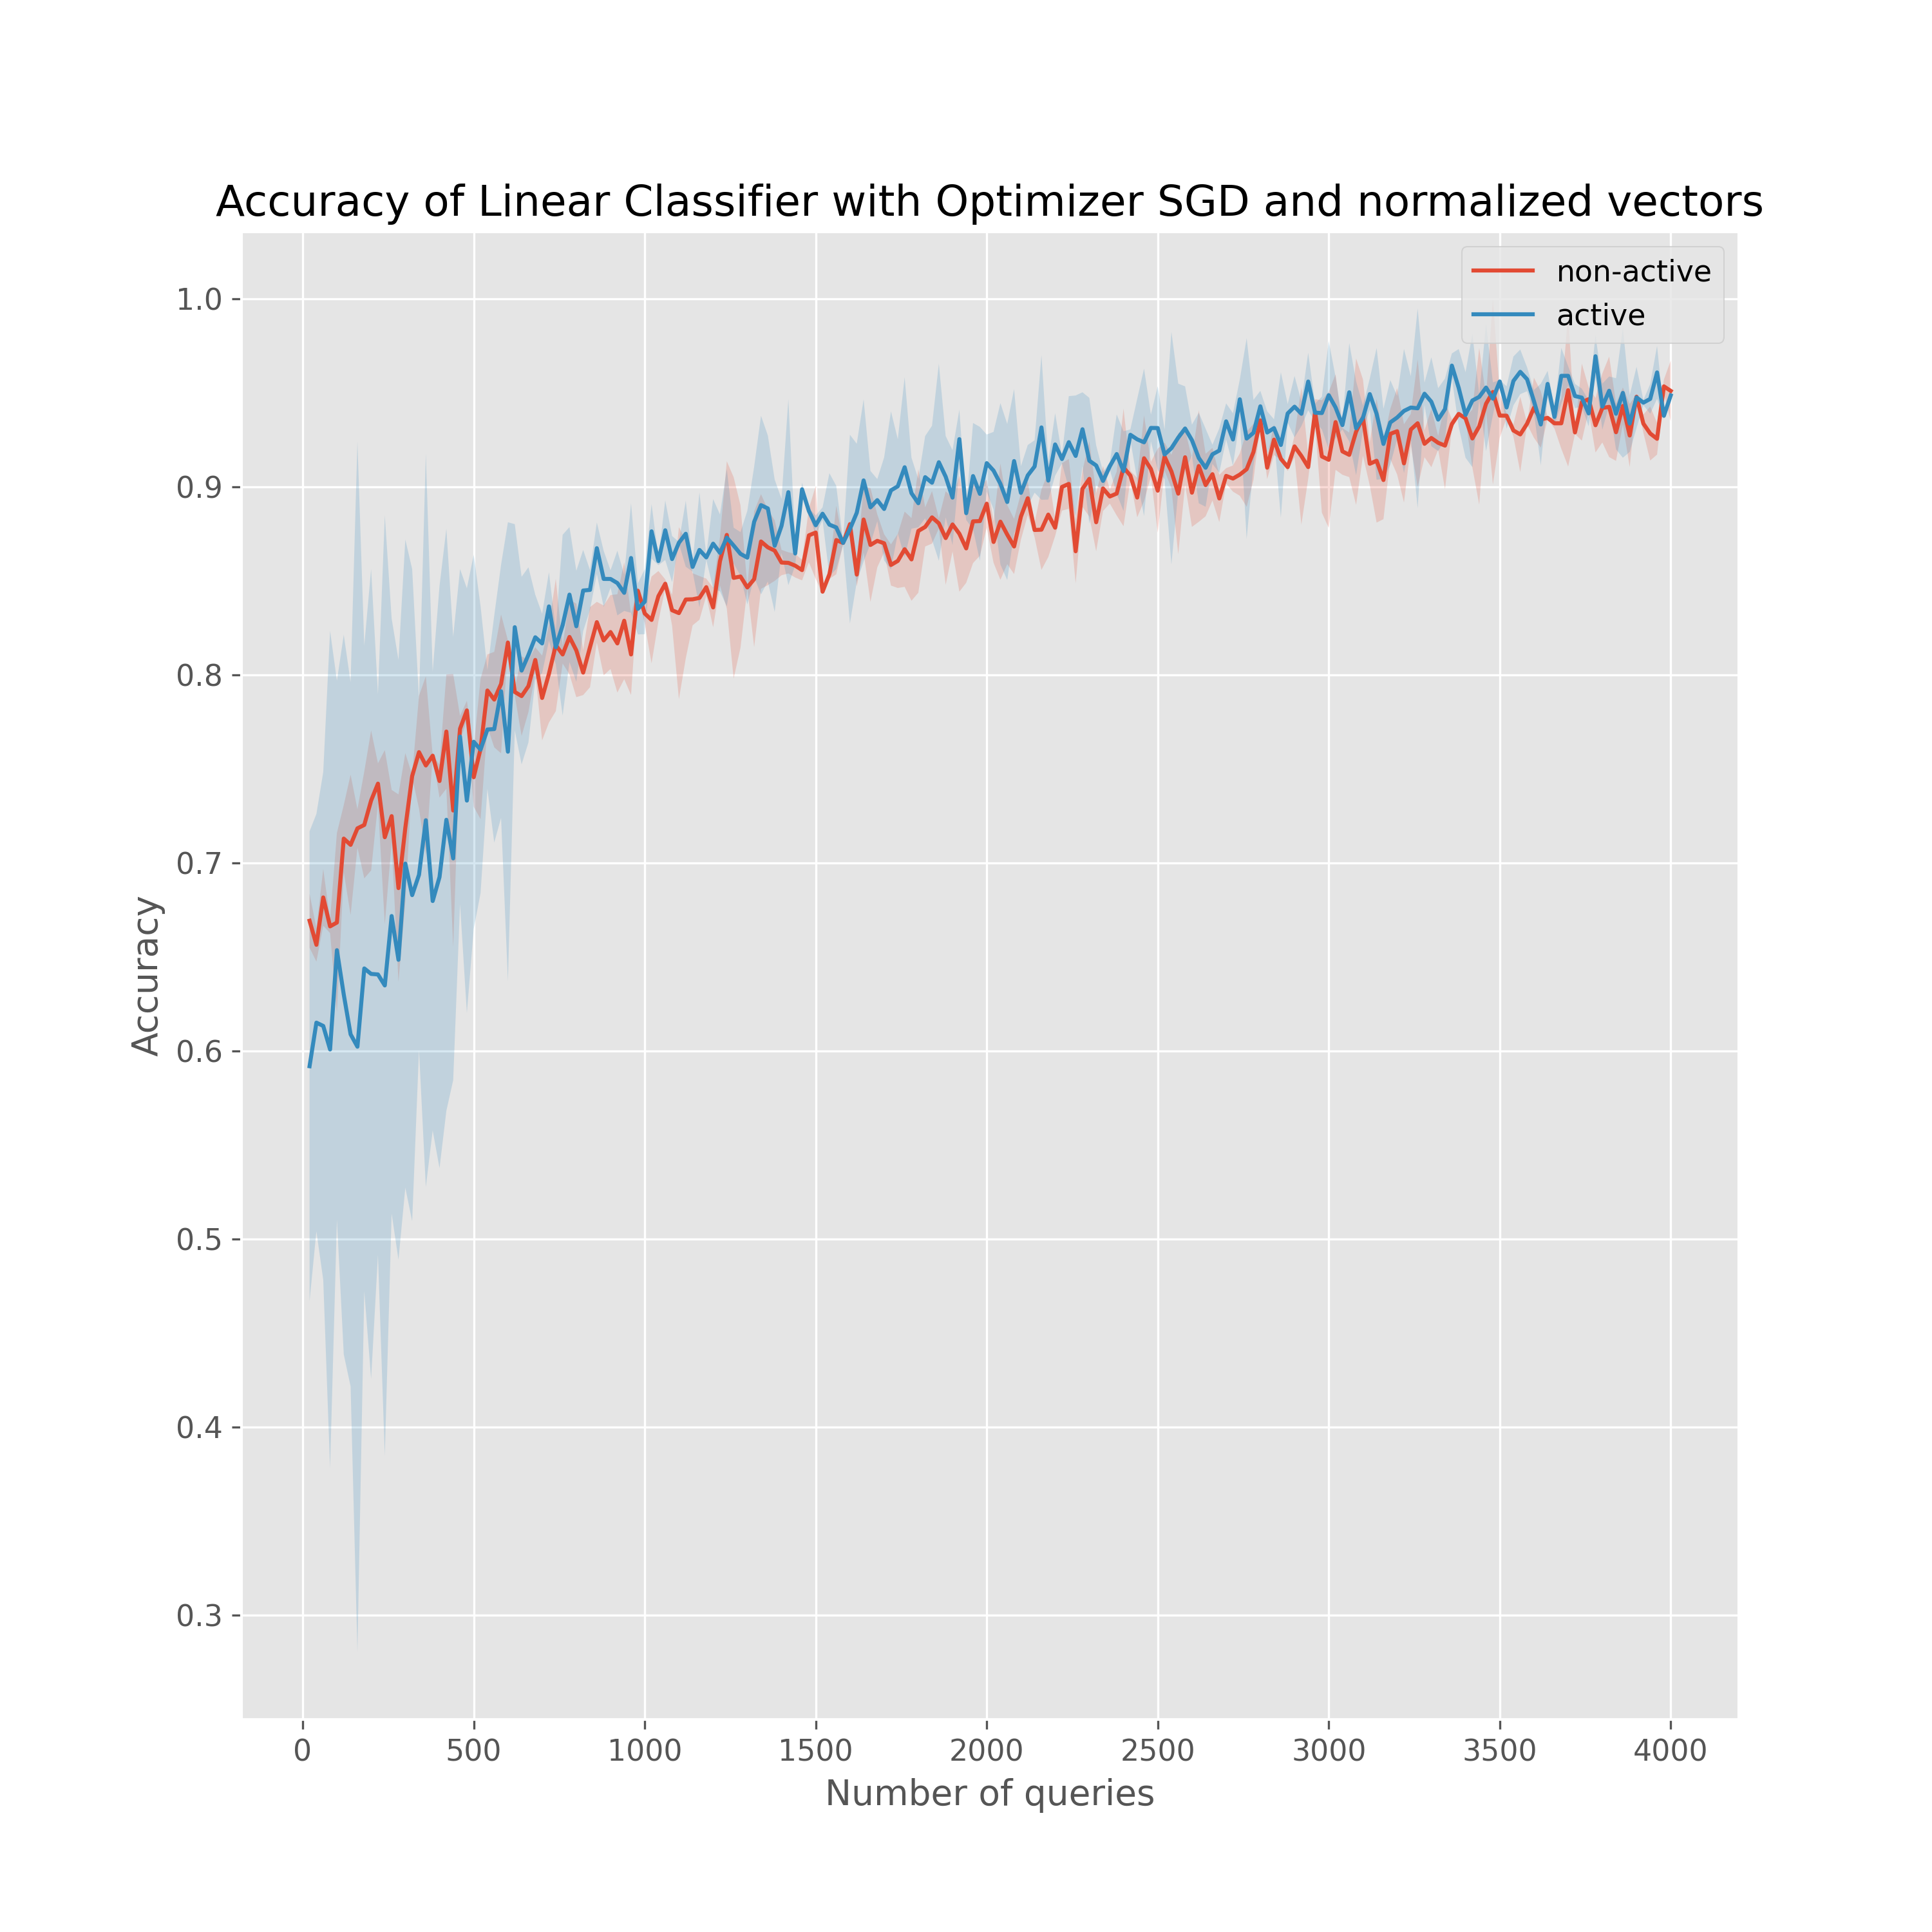
\includegraphics[width=\linewidth]{active-vs-base-moons-linear-loss-SGD-normalized-ci}
  \end{minipage}%
  \begin{minipage}{.55\textwidth}
    \centering
    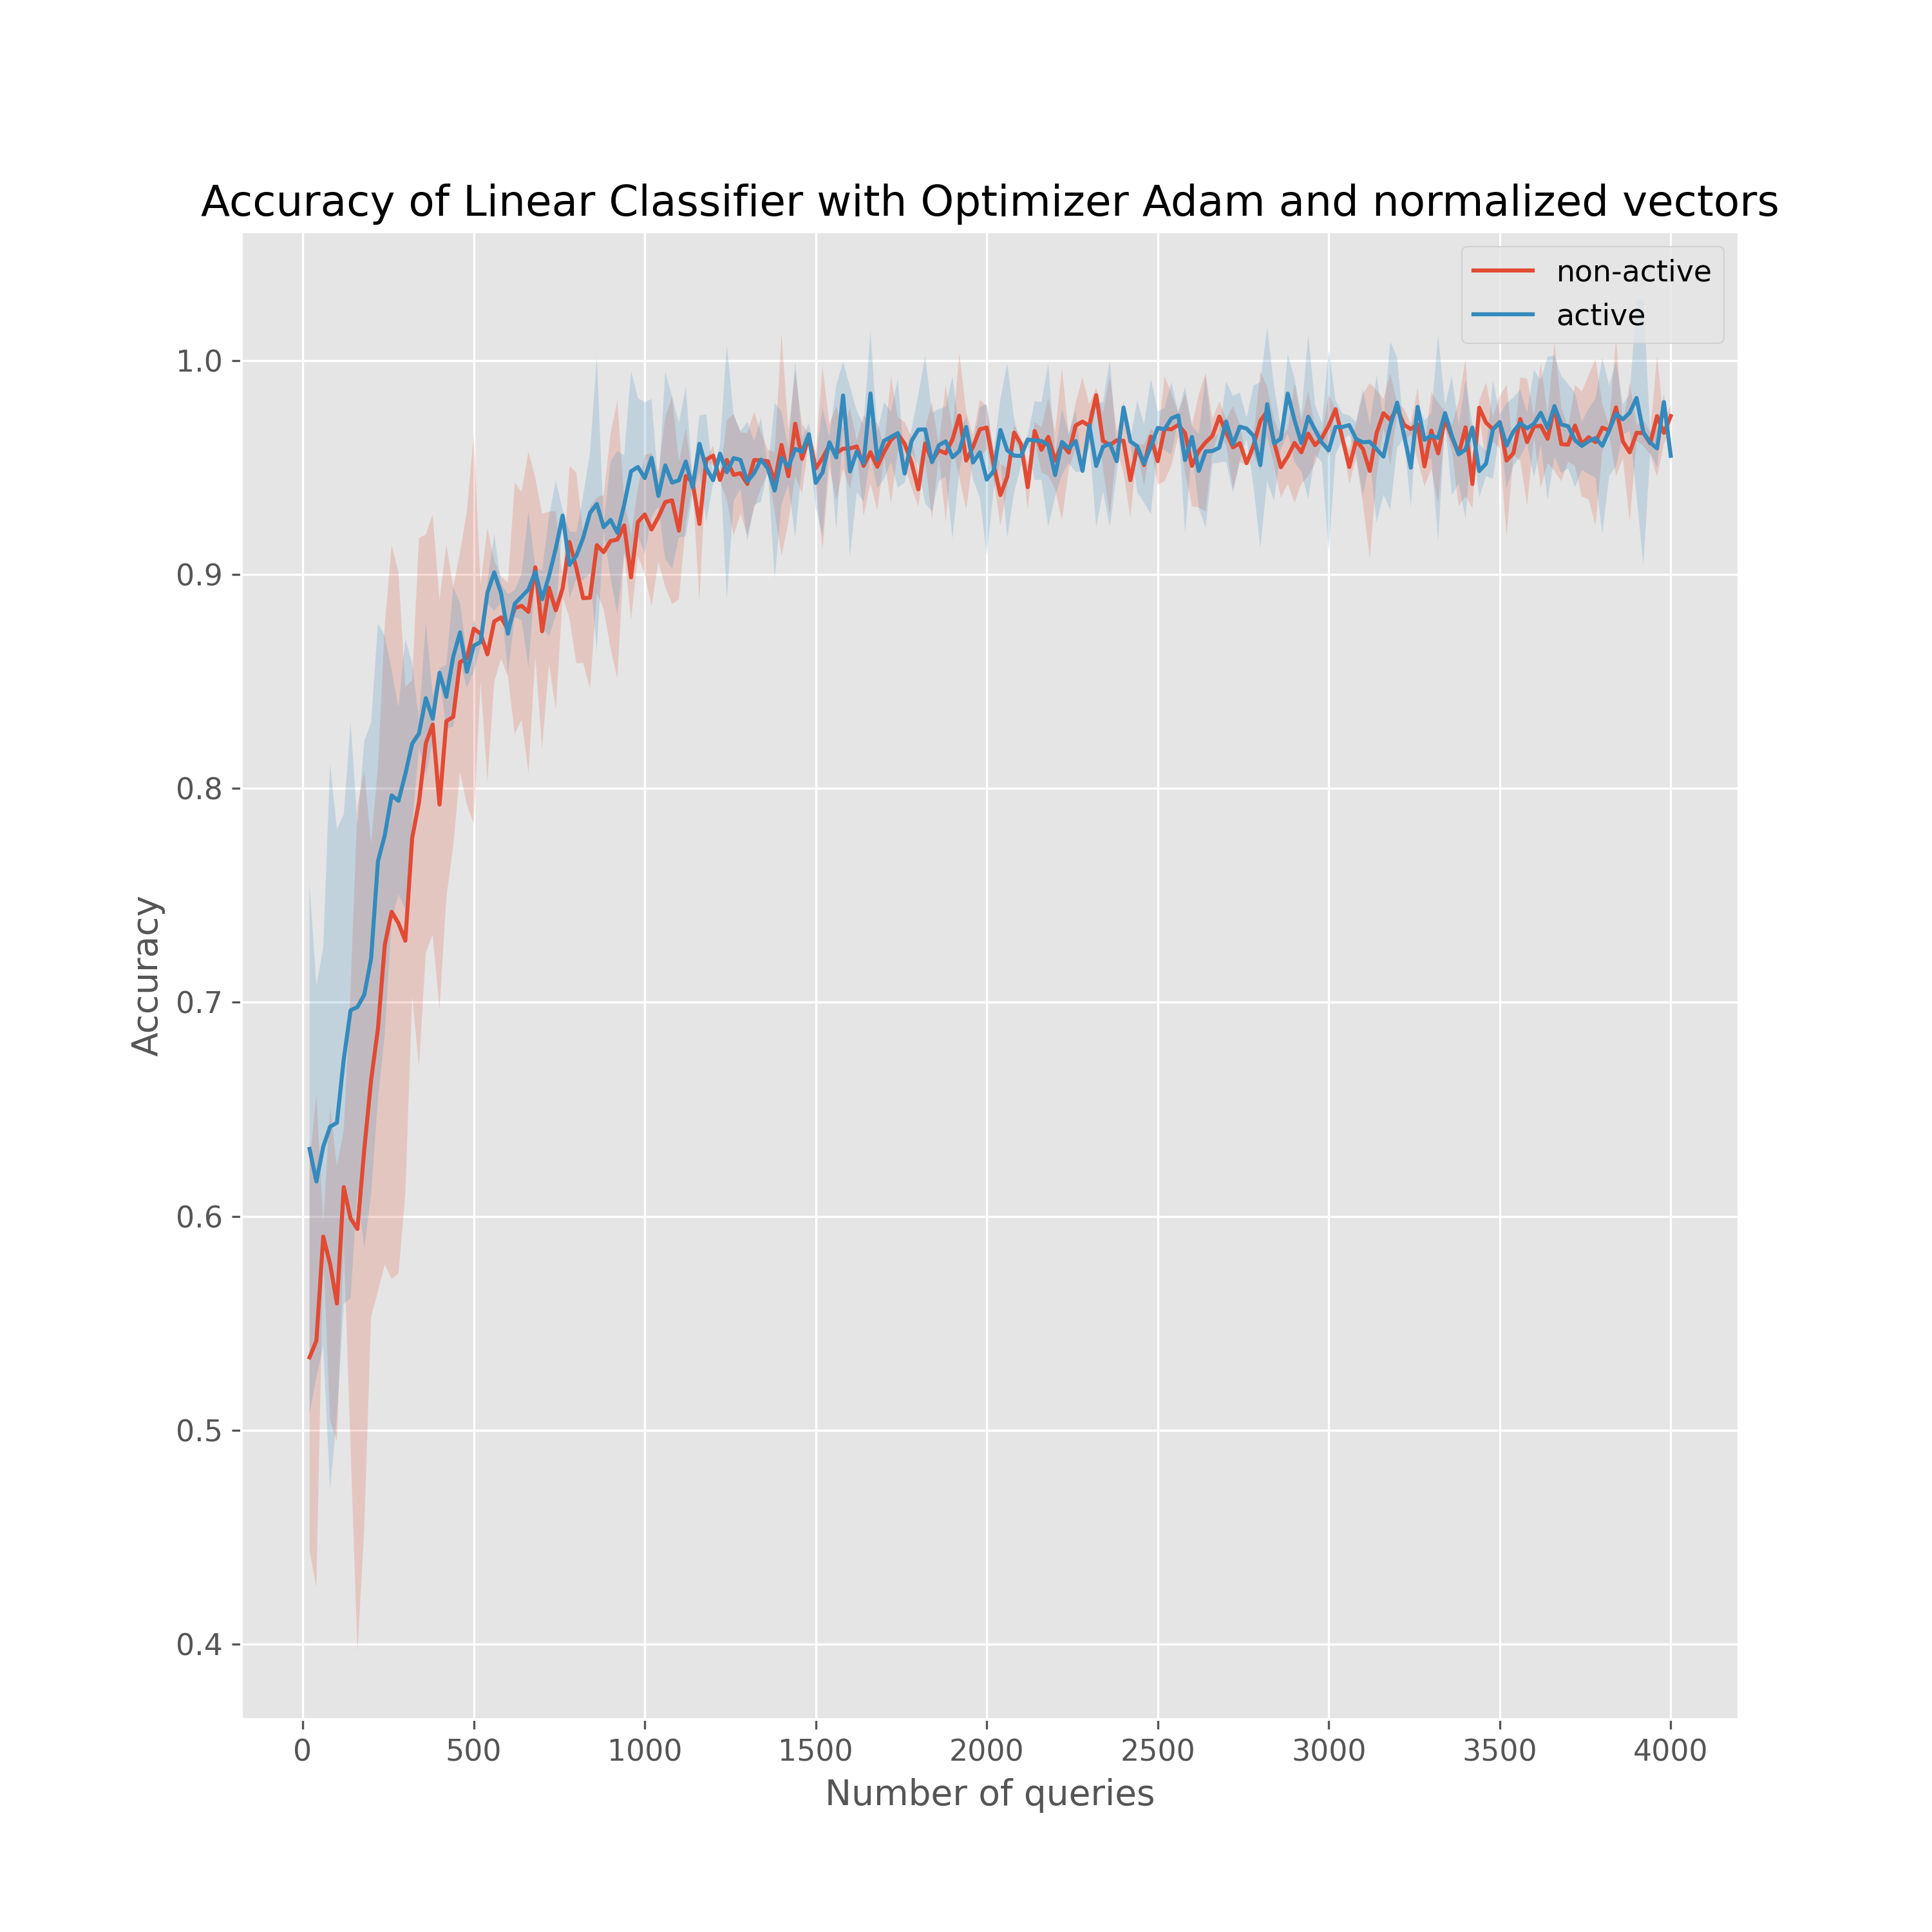
\includegraphics[width=\linewidth]{active-vs-base-moons-linear-loss-Adam-normalized-ci}
  \end{minipage}
  \caption{Performance SVM on normalzied learned features Adam vs SGD}
  \label{fig:svm-normalized-ci}
\end{figure}

\section{Conclusion}


\bibliography{refs}
\bibliographystyle{plain}

\end{document}
